% !TeX root = ../main.tex

\section{Base de Dados e Planejamento Experimental}

\subsection{Contexto do problema e medidas avaliadas}

A raça Nelore é originária da Índia, onde seus ancestrais, os bovinos da raças Ongole, eram criados há milênios por sua rusticidade, resistência a climas tropicais e capacidade de adaptação a ambientes variádos, esses animais foram trazidos ao Brasil no final do século XIX, em um momento de expansão da pecuária nacional \cite{hist_nelore}. A raça Caracu, por sua vez, tem origem na região da Península Ibérica,chegando no Brasil  logo após o descobrimento, os animais da raça Caracu são extremamente funcionais, com alta adaptabilidade e rusticidade, além de serem resistentes a doenças e parasitas \cite{hist_caracu}. O Brasil é um dos maiores criadores mundiais de bovinos da raça Nelore, com uma população estimada em mais de 230 milhões de cabeças \cite{embrapa1}, enquanto a raça Caracu é menos numerosa, mas ainda assim desempenha um papel importante na pecuária brasileira. 


Uma das principais formas de avaliar o desenvolvimento e a qualidade fenótipa dos animais é por meio da análise de imagens de ultrassonografia em que é possível obter informações da carcaça do animal. Entre os recursos e metodologias existentes para avaliação de carcaças e de características associadas à qualidade da carne, a ultrassonografia se destaca. A avaliação é de extrema importância pois existe uma variabilidade nas características que estão relacionadas com a qualidade de desossa, que por sua vez influenciam a comercialização e os resultados econômicos dos produtores \cite{cap3:nelore_caracu}.

Dependedo da região do corpo do animal onde a imagem de ultrassom é obtida, é possível extrair diferentes informações, neste trabalho serão utilizadas imagens de ultrassom da região do olho de lombo, que localiza-se entre a 12ª e 13ª costela \cite{cap3:carcaça} e da Garupa, como mostra a Figura \ref{fig:regiao_ol}. 

\begin{figure}[H]
    \centering
    \caption{Região do olho de lombo (em amarelo), localizada entre a 12ª e 13ª costela e da garupa (em azul).}
    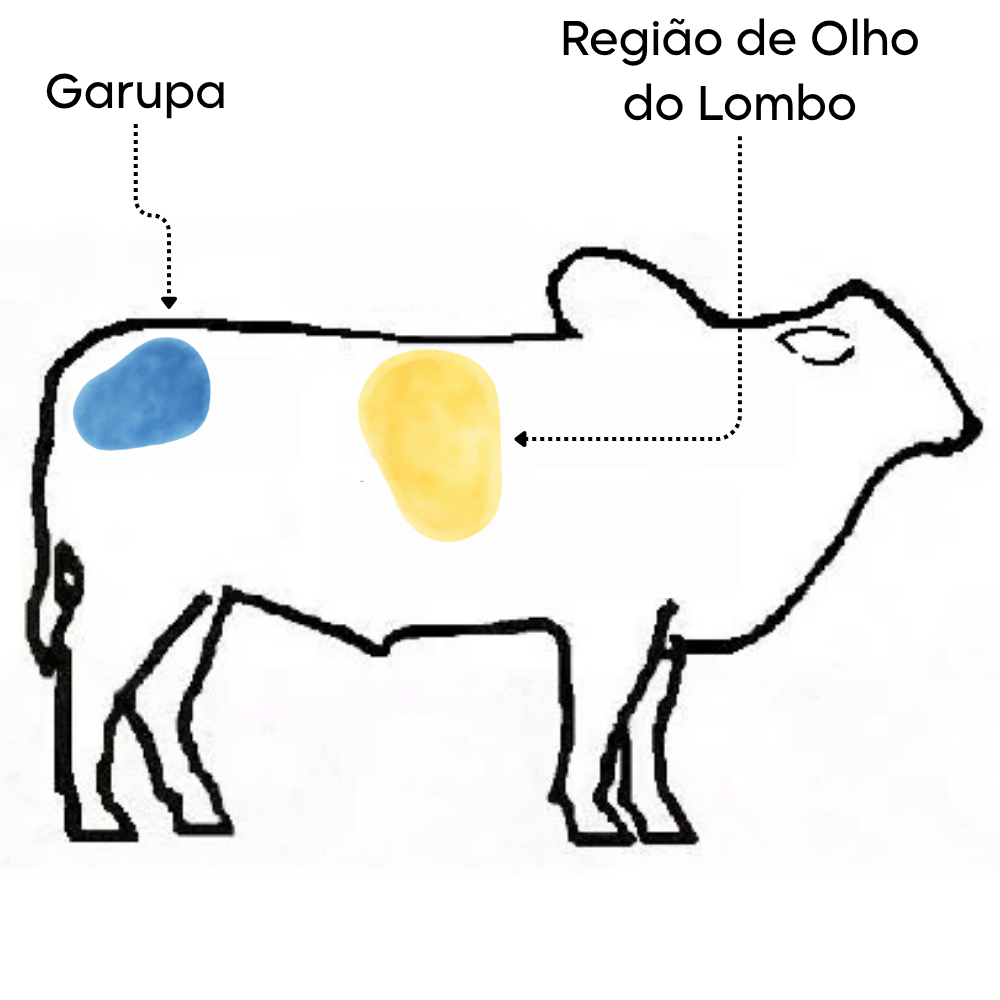
\includegraphics[width=0.5\textwidth]{figures/olho_lombo.png}
    \caption*{Fonte: Adaptado de \cite{cap3:carcaça}.}
    \label{fig:regiao_ol}
\end{figure}

Na região de olho do lombo é possível obter informações de duas medidas importantes para a avaliação da carcaça, a Área de Olho de Lombo (AOL) e a Espessura de Gordura no Lombo (EGL). Na Garupa é possível obter a informação da Espessura de Gordura na Garupa (EGG). As imagens de ultrassom foram obtidas por meio do aparelho de ultrassom Aloka SSD-500 \cite{AlokaSSD5001990}, com todos os animais sendo machos por volta de um ano de idade, localizados no Centro Avançado de Pesquisa Tecnológica do Agronegócio em Setãozinho-SP. A Figura \ref{fig1:OL}(a) mostra a imagem do especialista obtendo a imagem de ultrassom da região do olho de lombo, já a Figura \ref{fig1:OL}(b) mostra a imagem de ultrassom, a Figura \ref{fig1:OL}(c) mostra a imagem de ultrassom da garupa e a Figura \ref{fig1:OL}(d) mostra o especialista obtendo a imagem de ultrassom da garupa.

\textcolor{red}{esperando elas mandarem as imagens}
\begin{figure}[H]
    \centering
    \caption{Aquisição da imagem de ultrassom da região do olho de lombo.}
    \begin{subfigure}{0.4\textwidth}
        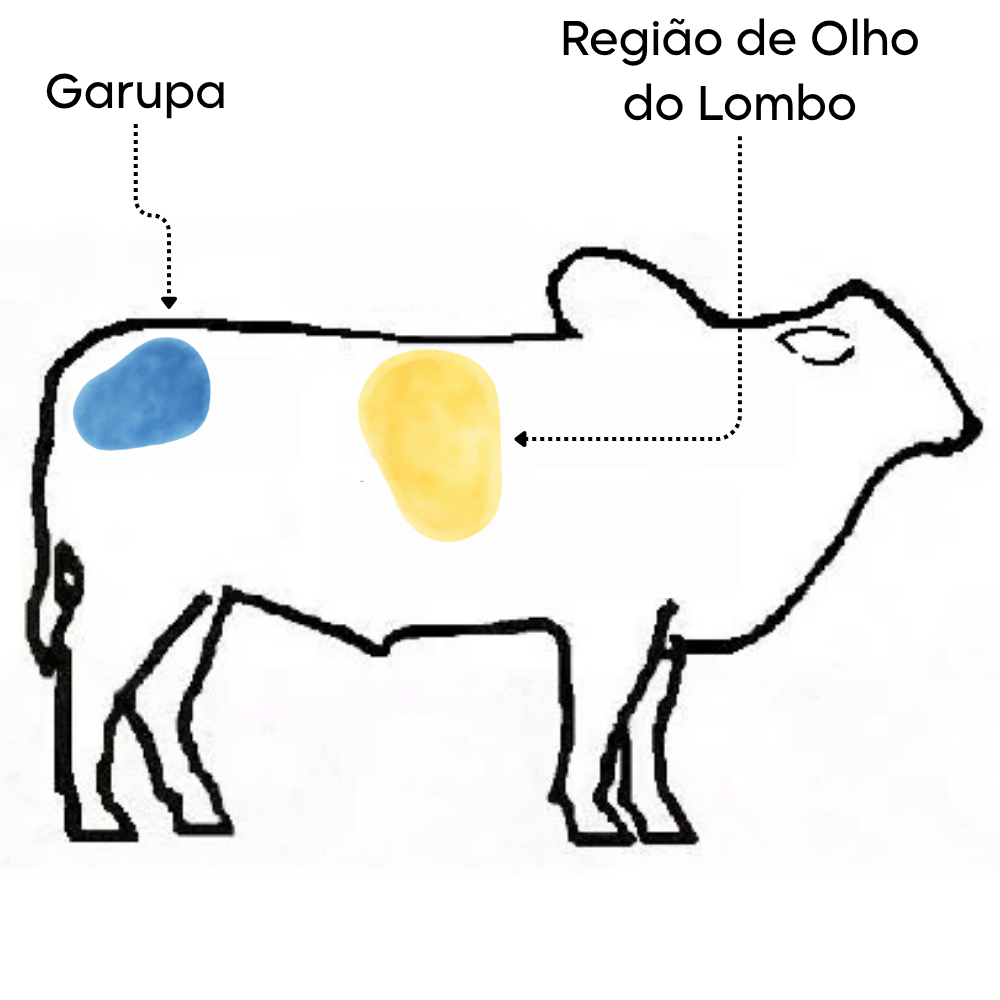
\includegraphics[width=\textwidth]{figures/olho_lombo.png}
        \caption{Especialista obtendo a imagem de ultrassom da região do olho de lombo.}
    \end{subfigure}
    \hfill
    \begin{subfigure}{0.4\textwidth}
        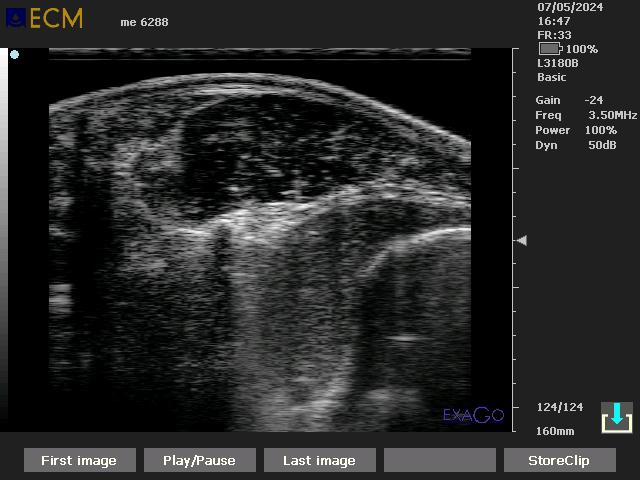
\includegraphics[width=\textwidth]{figures/OL.jpg}
        \caption{Imagem de ultrassom da região do olho de lombo.}
    \end{subfigure}
    \hfill
    \begin{subfigure}{0.4\textwidth}
        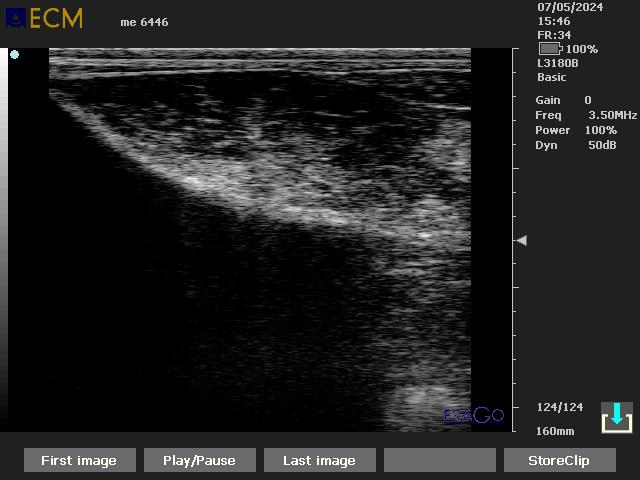
\includegraphics[width=\textwidth]{figures/cap3/EGG.jpg}
        \caption{Imagem de ultrassom da garupa.}
    \end{subfigure}
    \hfill
    \begin{subfigure}{0.4\textwidth}
        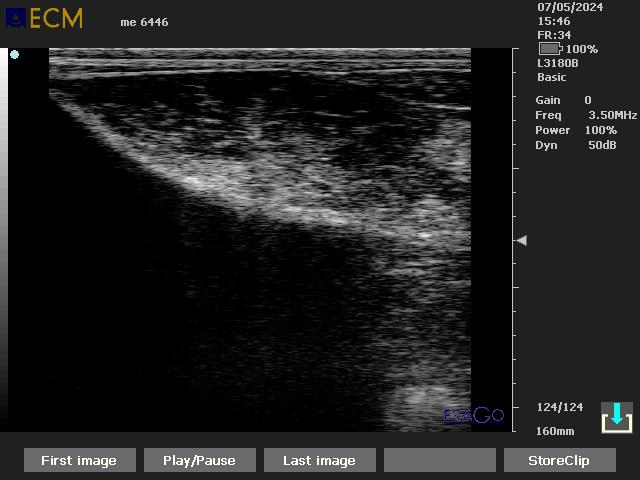
\includegraphics[width=\textwidth]{figures/cap3/EGG.jpg}
        \caption{Especialista obtendo a imagem de ultrassom da garupa.}
    \end{subfigure}
     \caption*{Fonte: Elaboração do Autor.}
     \label{fig1:OL}
\end{figure}

A área de olho de lombo é uma medida que representa a área da seção transversal do músculo  \textit{Longissimus dorsi} (Contrafilé), medida em centímetro quadrados entre a 12ª e 13ª costela. Uma maior área é preferível pelos produtores. Do ponto de vista produtivo, pode-se afirmar que animais com valores de AOL superiores a $75$ cm$^2$, ao abate, apresentam elevados rendimentos de cortes cárneos na indústria figorífica \cite{cap3:medidaAol}. Na Figura \ref{cap3:AOL} é mostrada a demarcação manual da área feita utilizando o aplicativo de manipulação e edição de imagens \textit{ImageJ} \cite{ImageJ} em que a região interna a demarção amarela é a AOL.
\begin{figure}[H]
    \centering
    \caption{Demarcação manual da Área de Olho de Lombo (AOL) utilizando o aplicativo \textit{ImageJ}.}
    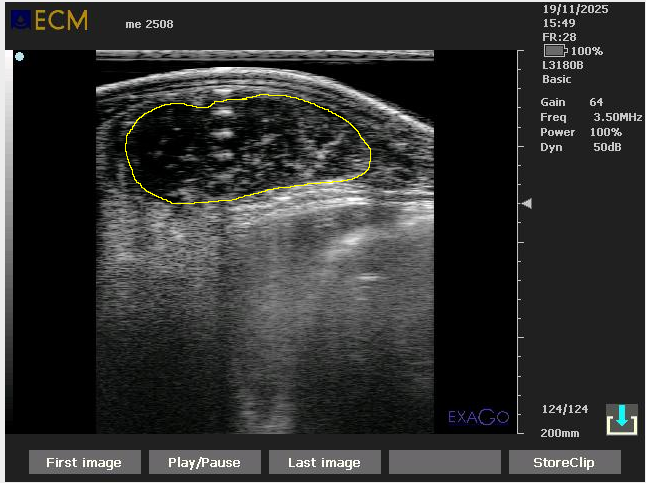
\includegraphics[width=0.7\textwidth]{figures/AOL.png}
    \caption*{Fonte: Elaboração do Autor.}
    \label{cap3:AOL}
\end{figure}

A espessura de gordura no lombo (EGL) é uma medida que representa a espessura da camada de gordura sobre o músculo \textit{Longissimus dorsi},  sendo sua espessura (EGL) medida, em milímetros, a $3/4$ da distância medial do músculo. Esta gordura de cobertura é extremamente importante para a proteção da carcaça contra a rápida e intensa queda de temperatura nas câmaras frias, que pode provocar o endurecimento (perda em maciez de até 5 vezes) e o escurecimento da carne em carcaças pobres em acabamento \cite{cap3:medidaAol}.

A EGL apresenta características antagônicas à AOL, ou seja, animais com maior deposição de gordura implicará em uma menor proporção de AOL na carcaça e menor peso ao abate \cite{cap3:medidaAol}. Na Figura \ref{cap3:EGL} é mostrada a demarcação manual feita no aplicativo \textit{ImageJ} em que a linha vermelha representa a demarcação da EGL. 

\begin{figure}[htpb]
    \centering
    \caption{Demarcação manual da Espessura de Gordura no Lombo (EGL) utilizando o aplicativo \textit{ImageJ}.}
    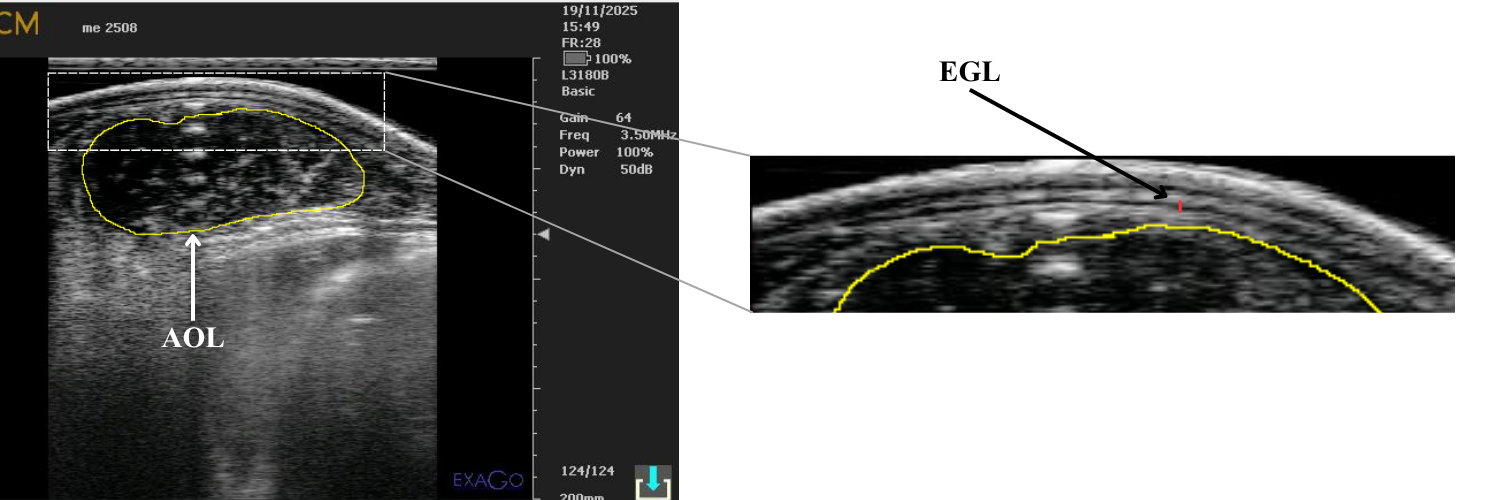
\includegraphics[width=1\textwidth]{figures/introducao/EGL.png}
    \caption*{Fonte: Elaboração do Autor.}
    \label{cap3:EGL}
\end{figure}

A espessura de gordura na garupa (EGG) é uma medida que representa a espessura da camada de gordura sobre a região da garupa, sendo medida em milímetros. A EGG é uma medida complementar à EGL, indicada principalmente para situações em que os animais têm a deposição de gordura subcutânea comprometida, principalmente por nutrição inadequada, como pode ocorrer, por exemplo, com animais em sistemas extensivos de pastejo \cite{cap3:medidaAol}. A medida é obtida no encontro do músculo \textit{Biceps Femoris}, comumente chamado de ponta da picanha, com a camada de gordura subcutânea \cite{cap3:carcaça}. Na Figura \ref{cap3:EGG} é mostrada a demarcação manual feita no aplicativo \textit{ImageJ}.

\begin{figure}[htpb]
   \centering
   \caption{Demarcação manual da Espessura de Gordura na Garupa (EGG) utilizando o aplicativo \textit{ImageJ}.}
   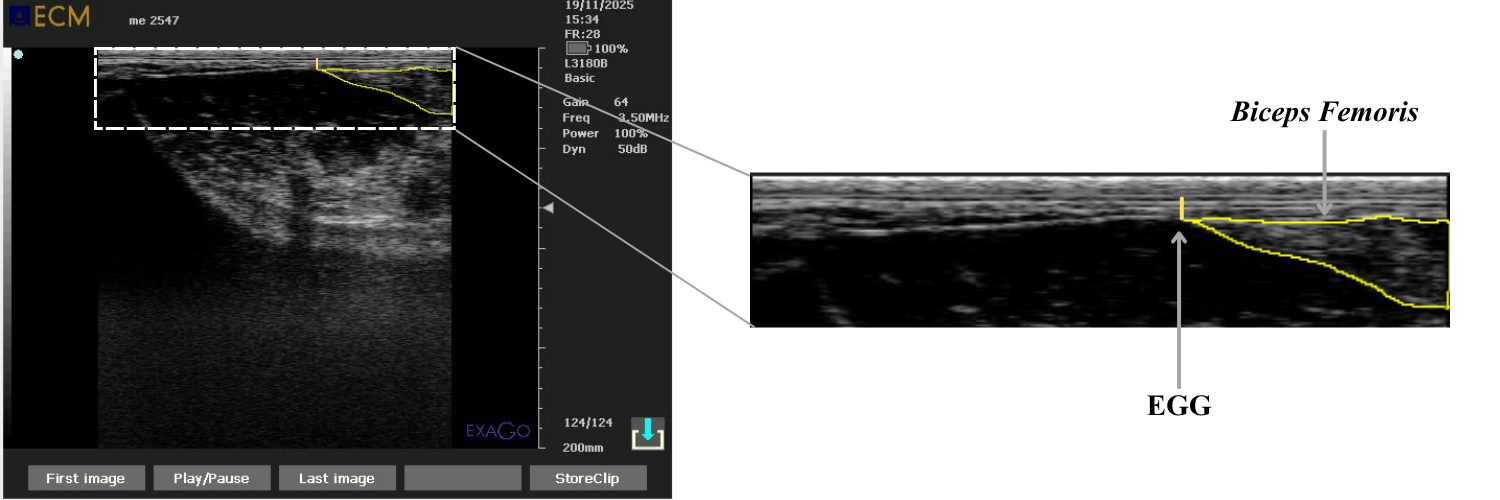
\includegraphics[width=1\textwidth]{figures/cap3/medidaEGG.png}
   \caption*{Fonte: Elaboração do Autor.}
   \label{cap3:EGG}
\end{figure}
A linha vertical amarela representa a demarcação da EGG. 


\subsection{Conjunto de dados}

O total de imagens enviadas pelo CAPTA com a delimitação do contorno da região feita por uma especialista foram 134 imagens de ultrassom (134 imagens da região de olho do lombo e 134 imagens da região da garupa), sendo 108 da raça Nelore e 27 da raça Caracu. Além das imagens enviadas, foram enviadas também as medidas numéricas correspondentes à delimitação da  AOL, EGL e EGG. As medidas foram enviadas em um arquivo do Excel, em que a primeria coluna continha o número de identificação do animal, a segunda coluna continha a medida da AOL, a terceira coluna continha a medida da EGL e a quarta coluna continha a medida da EGG. Essas medidas foram utilizadas para calcular o erro absoluto médio (MAE) entre as medidas preditas pelo modelo e as medidas reais. 

\subsection{Pré-processamento e Máscaras de Segmentação}

As imagens foram divididas em conjuntos de treinamento (70\%), validação (20\%) e teste (10\%). A biblioteca do Python, \textit{label studio} \cite{LabelStudioSite}, foi utilizada para criar as máscras de segmentação para as regiões correspondentes à AOL, EGL e EGG com base nas delimitações das regiões feitas pela especialista. Foram utilizadas como ``rótulos", ou seja, cada imagem do banco de dados tinha uma máscara correspondente. Devido a pequena quantidade de imagens para o treinamento de um modelo de aprendizado profundo, foi necessário aplicar um processo de aumento de dados, do inglês \textit{data augmentation}, para ampliar o conjunto de imagens utilizado no treinamento. Além disso, foi realizado um recorte nas imagens para remover informações irrelevantes, que poderiam introduzir vieses no treinamento e comprometer o desempenho dos modelos. O processo de aumento de dados incluiu as seguintes transformações:
\begin{itemize}
    \item Rotação: As imagens foram rotacionadas em ângulos dentro do intervalo de $[-15^\circ, 15^\circ]$ para criar variações na orientação das imagens.
    \item Aumento e redução de brilho: As imagens foram aumentadas e reduzidas em brilho para simular diferentes condições de iluminação.
\end{itemize}
Todas as modificações feitas foram realizadas observando as características das imagens de ultrassom presentes no banco de dados. Como cada imagem foi modificada tres vezes, o processo de aumento de dados resultou em um total de $372$ imagens para o treinamento do modelo (adicionando também as imagens originais). Após o aumento de dados, as imagens foram normalizadas, com os valores dos pixels ajustados para o intervalo $[0, 1]$, e redimensionadas para um tamanho fixo de $256 \times 256$\footnote{As imagens após o corte inicial tinham dimensões de 333x403, a escolha de 256x256 foi feita para que a imagem não fosse muito expandida (aumento de pixels) e que não perdesse muita resolução (diminuição de pixels). Outros testes foram feitos para resolusões diferentes que resultaram em um desempenho inferior.} pixels.  Na Figura \ref{cap3:preprocessamento} é mostrado o processo de pré-processamento de uma imagem.
\begin{figure}[H]
    \centering
    \caption{Exemplo do processo de pré-processamento das imagens de ultrassom.}
    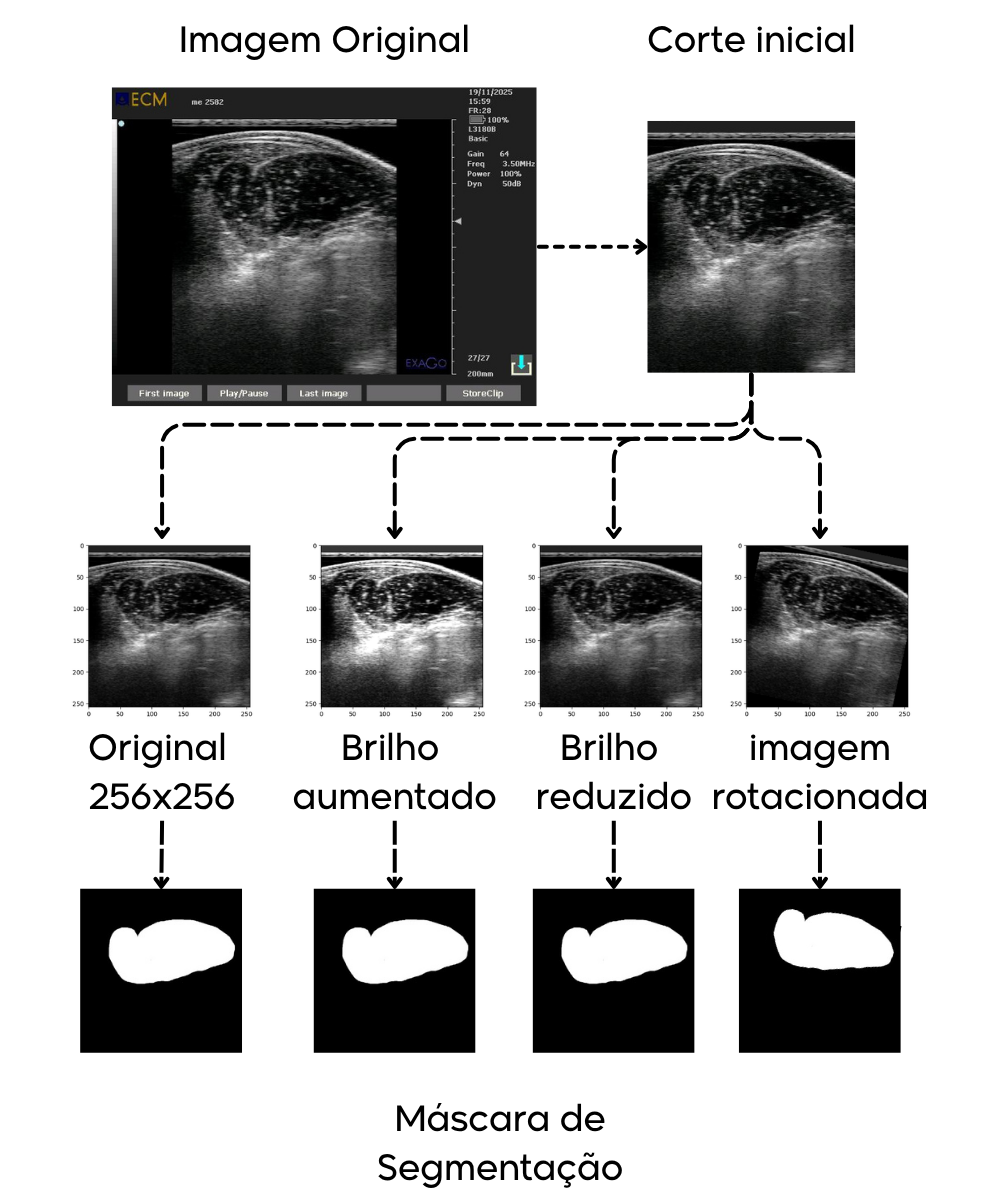
\includegraphics[width=0.6\linewidth]{figures/cap3/augmentation.png}  
    \caption*{Fonte: Elaboração do Autor.}
    \label{cap3:preprocessamento}  
\end{figure}
Na Figura \ref{cap3:preprocessamento} uma imagem é pré-processada e a máscara de segmentação correspondente a medida de AOL é criada para cada nova imagem adicionada, observa-se que a imagem rotacionada mantém consistência com a máscara, ou seja, a máscara acompanha corretamente a rotação da imagem.

Cada medida extraída nas imagens de ultrassom (AOL, EGL e EGG) são números reais. Uma ideia inicial foi desenvolver uma CNN (\ref{redesConvolucionais}) que recebia como entrada as imagens de ultrassom e retornava como saída os valores numéricos correspondentes à AOL, EGL e EGG, ou seja, uma rede de regressão. No entanto, devido à quantidade baixa de imagens disponíveis para o treinamento do modelo, foi necessário realizar uma adaptação na abordagem inicial. Em vez de treinar uma CNN para prever os valores numéricos das medidas, optou-se, após análise literária, por criar máscaras de segmentação para cada medida (AOL, EGL e EGG) a partir das imagens de ultrassom  \cite{JadersonMelo2022UNetpp}. As máscaras de segmentação foram criadas a apartir das delimitações feitas pela especialista. 

Os modelos desenvolvidos recebem a imagem de ultrassom como entrada e fazem um processo de segmentação da imagem, gerando como saída uma máscara de segmentação. Cada medida (AOL, EGL e EGG) tem uma máscara de segmentação correspondente, uma para a AOL, uma para a EGL e duas para a EGG. Como a medida da EGG é obtida a partir da espessura da camada de gordura sobre o músculo \textit{Biceps Femoris}, foram criadas duas máscaras de segmentação para a EGG, uma para a camada de gordura e outra para o músculo \textit{Biceps Femoris}. Por conta disso foram desenvolvidos e treinados oito modelos diferentes, quatro modelos U-Net multitarefa e quatro modelos U-Net Fuzzy. Após o treinamento, a saída de cada modelo é uma máscara de segmentação, a partir dessa máscara é possível extrair as medidas numéricas correspondentes à AOL, EGL e EGG. Para a AOL, a medida é obtida a partir da contagem do número de pixels classificados como pertencentes a região de interesse (pixel brancos) e convertida para centímetros quadrados. 
Para EGL, os pixels pertencentes à região de interesse são contados e convertidos em milímetros, com isso é possível obter a largura da camada de gordura, a $3/4$ desta largura é obtida a altura da camada de gordura, que é a medida da EGL. Para a EGG, como duas máscaras são criadas por dois modelos diferentes, quando uma imagem é enviada e processada pelos modelos, um retorna a máscara de segmentação da camada de gordura presente na Garupa e o outro retorna a máscara de segmentação do músculo \textit{Biceps Femoris}. A partir dessas duas máscaras é possível obter a medida da EGG, primeiramente salvando a localização da coluna que se inicia o músculo \textit{Biceps Femoris} (da esquerda para a direita) na segunda máscara e calculando a espessura da gordura na primeira máscara presente na mesma coluna, ou seja, a espessura da camada de gordura na garupa é medida na gordura que fica sobre o começo do músculo \textit{Biceps Femoris}. Na Figura \ref{cap3:mascaras} é mostrado um exemplo das máscaras de segmentação criadas para as imagens de ultrassom.
\begin{figure}[htpb]
    \centering
    \caption{Exemplo das máscaras de segmentação criadas para as imagens de ultrassom.}
    \begin{subfigure}{0.45\textwidth}
        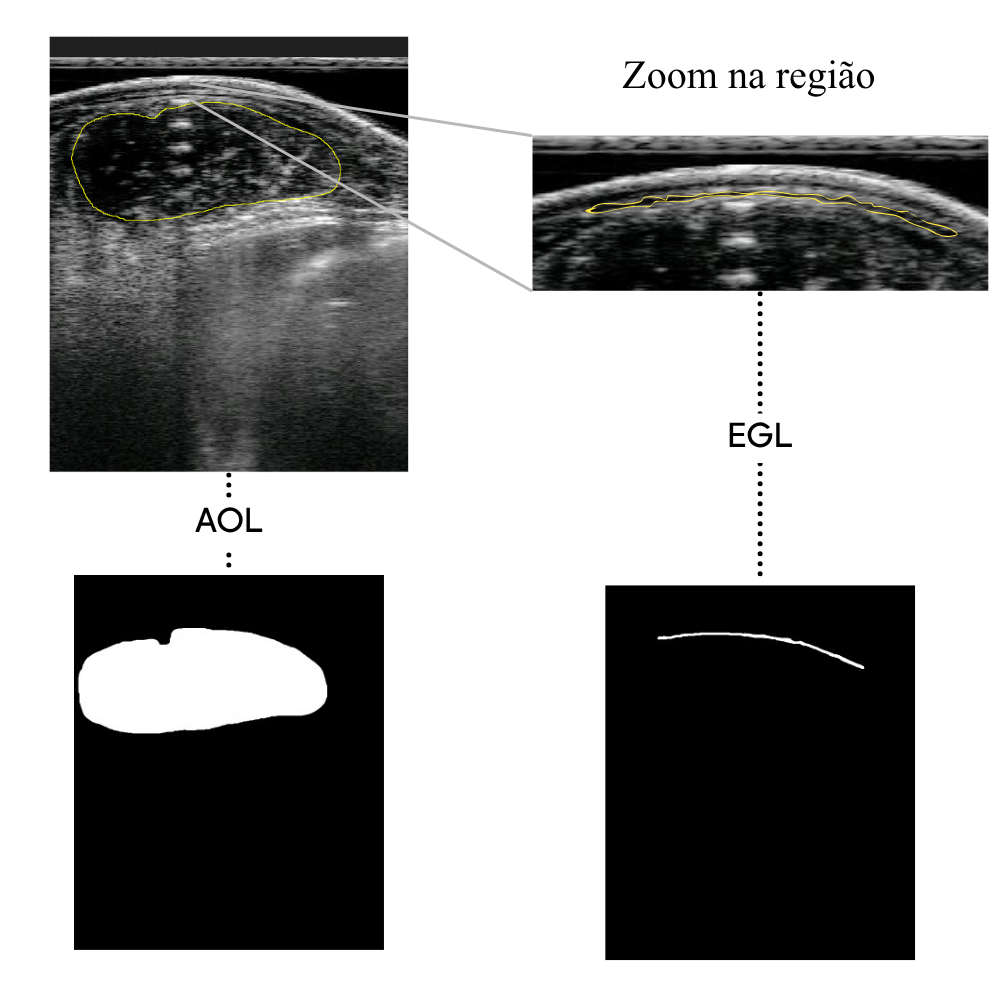
\includegraphics[width=\textwidth]{figures/cap3/mascaras.png}
        \caption{Segmentação da AOL e EGL na região do olho de lombo.}
    \end{subfigure}
    \hfill
    \begin{subfigure}{0.45\textwidth}
        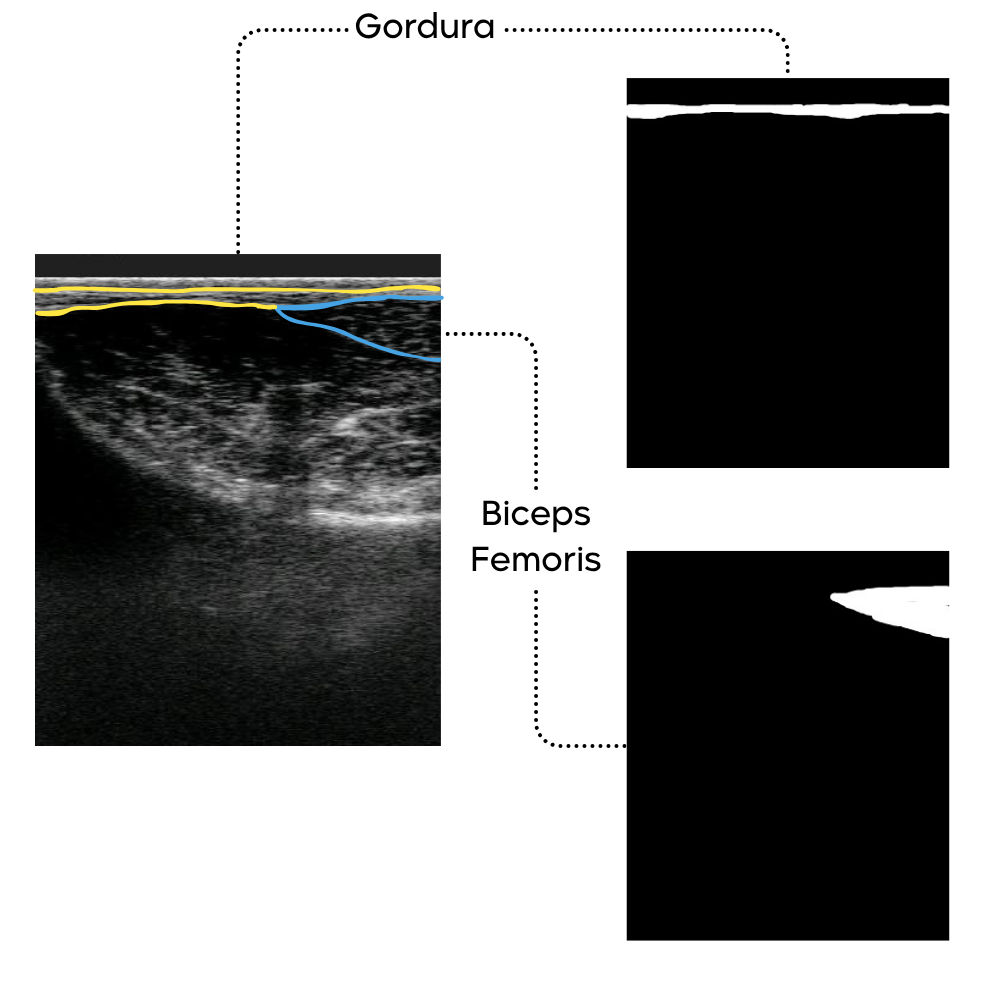
\includegraphics[width=\textwidth]{figures/cap3/mascaras2.png}
        \caption{Segmentação da EGG na região da garupa.}
    \end{subfigure}
     \caption*{Fonte: Elaboração do Autor.}
     \label{cap3:mascaras}
\end{figure}

Na Figura \ref{cap3:mascaras}(a) é mostrada a delimitação da região feita pela especialista e a respectiva máscara de segmentação. Na Figura \ref{cap3:mascaras}(b) é mostrada a delimitação da região feita pela especialista e as respectivas máscaras de segmentação, a máscara superior é a máscara de segmentação da camada de gordura e a máscara inferior é a máscara de segmentação do músculo \textit{Biceps Femoris}. Cada imagem de animal presente no banco de dados vinha com um número de indentificação. Animais com o primeiro dígito começando em $6$, são animais da raça Nelore, enquanto animais com o primeiro dígito começando em $2$, são animais da raça Caracu. Essa indentificação serviu para terminar o desenvolvimento do banco de dados e criar como abordado na seção \ref{multitask}.


\section{Configuração dos Modelos}

Esta seção descreve os procedimentos adotados para a comparação experimental entre os modelos propostos. Como os fundamentos teóricos, as arquiteturas e a formulação matemática das métricas já foram apresentados no Capítulo 3, o foco desta seção recai sobre os modelos comparados, a configuração de treinamento, as métricas utilizadas na avaliação e o ambiente computacional empregado nos experimentos.

\subsection{Modelos comparados}

Foram comparadas duas arquiteturas para a segmentação das imagens de ultrassom: a U-Net multitarefa e a U-Net Fuzzy. A U-Net multitarefa incorpora, no \textit{baseline} da rede, a informação categórica da raça do animal, enquanto a U-Net Fuzzy mantém essa estrutura e adiciona uma camada de inferência fuzzy baseada em ANFIS, conforme descrito no Capítulo 3. Em ambas as arquiteturas, a entrada do modelo é composta pela imagem de ultrassom e pela codificação da raça do animal no formato \textit{One-Hot Encoding}.

A comparação foi realizada separadamente para cada tarefa de segmentação associada às medidas avaliadas. Para a AOL e a EGL, foi treinado um modelo de cada arquitetura. Para a EGG, devido à necessidade de identificar simultaneamente a camada de gordura e o músculo \textit{Biceps Femoris}, foram treinados dois modelos por arquitetura, um para cada estrutura anatômica. Assim, no total, foram avaliados oito modelos.

\begin{table}[H]
    \centering
    \caption{Quantidade de modelos desenvolvidos para cada medida.}
    \begin{tabular}{|l|c|c|}
        \hline
        \textbf{Tarefa de segmentação} & \textbf{U-Net multitarefa} & \textbf{U-Net Fuzzy} \\
        \hline
        AOL & 1 & 1 \\
        \hline
        EGL & 1 & 1 \\
        \hline
        EGG - camada de gordura & 1 & 1 \\
        \hline
        EGG - músculo \textit{Biceps Femoris} & 1 & 1 \\
        \hline
        Total & 4 & 4 \\
        \hline
    \end{tabular}
    \caption*{Fonte: Elaboração do Autor.}
    \label{tab:modelos_comparados}
\end{table}

\subsection{Configuração de treinamento}

Todos os modelos foram treinados a partir das imagens previamente recortadas, normalizadas no intervalo $[0,1]$ e redimensionadas para $256 \times 256$ pixels. As imagens destinadas ao treinamento foram submetidas ao processo de aumento de dados descrito anteriormente, com o objetivo de ampliar a variabilidade do conjunto amostral e reduzir o risco de sobreajuste.

A configuração de treinamento foi mantida, em sua maior parte, idêntica para as duas arquiteturas, a fim de tornar a comparação entre os modelos mais consistente. Em ambos os casos, foi utilizado o otimizador Adam, com taxa de aprendizado inicial de $0{,}001$, tamanho de lote igual a $4$, número máximo de $100$ épocas e função de custo \textit{Binary Cross-Entropy}. Além disso, foram empregadas camadas de \textit{Dropout} com taxa de $0{,}2$ e o critério de \textit{EarlyStopping}, com base no desempenho no conjunto de validação, para reduzir a ocorrência de \textit{overfitting}.

Para a U-Net Fuzzy, além dessa configuração comum, foram definidos $3$ conjuntos fuzzy para a variável de entrada do módulo de inferência e $9$ regras fuzzy, considerando as combinações possíveis entre os conjuntos. Para reduzir o efeito da aleatoriedade inerente ao processo de treinamento, cada modelo foi treinado quatro vezes, sendo os resultados apresentados na próxima seção uma média dos valores obtidos.

\begin{table}[H]
    \centering
    \caption{Resumo da configuração de treinamento adotada nos experimentos.}
    \begin{tabular}{|l|l|}
        \hline
        \textbf{Parâmetro} & \textbf{Valor} \\
        \hline
        Tamanho da imagem de entrada & $256 \times 256$ pixels \\
        \hline
        Normalização & intervalo $[0,1]$ \\
        \hline
        Otimizador & Adam \\
        \hline
        Taxa de aprendizado inicial & $0{,}001$ \\
        \hline
        Tamanho do lote & $4$ \\
        \hline
        Número máximo de épocas & $100$ \\
        \hline
        Função de custo & \textit{Binary Cross-Entropy} \\
        \hline
        \textit{Dropout} & $0{,}2$ \\
        \hline
        Critério de parada & \textit{EarlyStopping} \\
        \hline
        Número de execuções por modelo & $4$ \\
        \hline
        Conjuntos fuzzy & $3$ \\
        \hline
        Regras fuzzy & $9$ \\
        \hline
    \end{tabular}
    \caption*{Fonte: Elaboração do Autor.}
    \label{tab:config_treinamento}
\end{table}

\subsection{Métricas de avaliação}

O desempenho dos modelos foi analisado sob duas perspectivas complementares: a qualidade da segmentação gerada e a precisão das medidas numéricas extraídas a partir das máscaras preditas.

No contexto da segmentação, foi adotado o coeficiente de Dice como principal métrica de avaliação, por quantificar diretamente a sobreposição entre a máscara predita pelo modelo e a máscara de referência elaborada pela especialista. A acurácia foi utilizada como métrica complementar, permitindo observar a proporção global de pixels classificados corretamente. Também foram analisados o comportamento da função de custo ao longo das épocas e o número de épocas necessárias até a convergência, como indicadores da estabilidade do processo de treinamento.

No contexto da mensuração das características da carcaça, foram utilizadas a reta de regressão linear, o coeficiente de determinação ($R^2$) e o erro absoluto médio (\textit{Mean Absolute Error} - MAE). O coeficiente $R^2$ foi empregado para avaliar o grau de associação entre as medidas preditas pelos modelos e as medidas fornecidas pela especialista, enquanto o MAE foi utilizado para quantificar, em unidade física, a magnitude média do erro entre os valores estimados e os valores de referência. Dessa forma, a combinação dessas métricas permitiu avaliar não apenas a capacidade dos modelos em segmentar corretamente as regiões de interesse, mas também sua utilidade prática na obtenção das medidas AOL, EGL e EGG.

\subsection{Ambiente computacional}

Os experimentos foram conduzidos em um notebook Asus TUF \textit{Gaming} F15, equipado com processador Intel Core i7-12700H, $8$ GB de memória RAM, unidade SSD de $512$ GB e placa de vídeo NVIDIA GeForce RTX 3050 Mobile com $4$ GB de memória dedicada. O sistema operacional utilizado foi o Linux Mint 22.3 ``Zena'' \cite{LinuxMintSite}.

A implementação dos modelos foi realizada na linguagem Python, versão 3.11.15 \cite{python}, com uso das bibliotecas TensorFlow 2.21.0, com suporte a GPU, e Keras 3.13.2 \cite{TensorFlowSite, KerasSite}. O desenvolvimento foi realizado no ambiente Visual Studio Code \cite{VSCodeSite}. O treinamento das redes neurais foi executado com aceleração por GPU, o que contribuiu para reduzir o tempo computacional necessário para a realização dos experimentos.


\section{Resultados e Análise}

Esta seção apresenta os resultados obtidos pelos modelos U-Net multitarefa e U-Net Fuzzy para a segmentação das imagens de ultrassom e para a mensuração das características AOL, EGL e EGG. Para cada medida, são analisados o desempenho de segmentação, a correspondência entre os valores preditos e as medidas de referência fornecidas pela especialista, bem como a comparação entre as duas arquiteturas. Os valores apresentados correspondem à média de quatro execuções independentes de cada modelo.
\subsection{AOL}
\subsubsection{U-Net multitarefa}

Para a mensuração da AOL, o modelo U-Net multitarefa apresentou bom desempenho na tarefa de segmentação. No conjunto de validação, obteve coeficiente de Dice médio de $92,73\%$ e acurácia média de $94,75\%$, indicando elevada sobreposição entre as máscaras preditas e as máscaras de referência. Em média, a convergência do treinamento ocorreu após $80$ épocas.

Em relação às medidas numéricas, o modelo alcançou erro absoluto médio (MAE) de $2,988$ cm$^2$ e coeficiente de determinação $R^2$ igual a $0,5578$. Esse resultado indica que, embora o modelo tenha segmentado adequadamente a região de interesse, a correspondência entre as medidas preditas e as medidas reais foi moderada. No conjunto de teste, o erro máximo observado foi de $7,905$ cm$^2$, o erro mínimo foi de $0,005$ cm$^2$, a média predita foi de $39,880$ cm$^2$ e a média real foi de $40,559$ cm$^2$.

A Figura \ref{cap3:metricasAOL}(a) apresenta a relação entre as medidas preditas e as medidas reais da AOL. Observa-se que os pontos acompanham a reta identidade, embora com dispersão compatível com o valor moderado de $R^2$. Já a Figura \ref{cap3:metricasAOL}(b) mostra o comportamento da função de custo, da acurácia e do coeficiente de Dice ao longo do treinamento. A função de custo reduziu até valores próximos de $0,09$, enquanto as curvas de acurácia e Dice apresentaram comportamento relativamente estável entre treinamento e validação. Embora haja indícios de \textit{overfitting} a partir de aproximadamente $20$ épocas, o modelo manteve capacidade de generalização satisfatória.

\begin{figure}[htpb]
    \centering
    \caption{Reta de regressão linear e $R^2$ entre as medidas preditas e as medidas reais da AOL e gráficos de custo, \textit{Dice} e acurácia ao longo das épocas.}
    \begin{subfigure}{0.45\textwidth}
        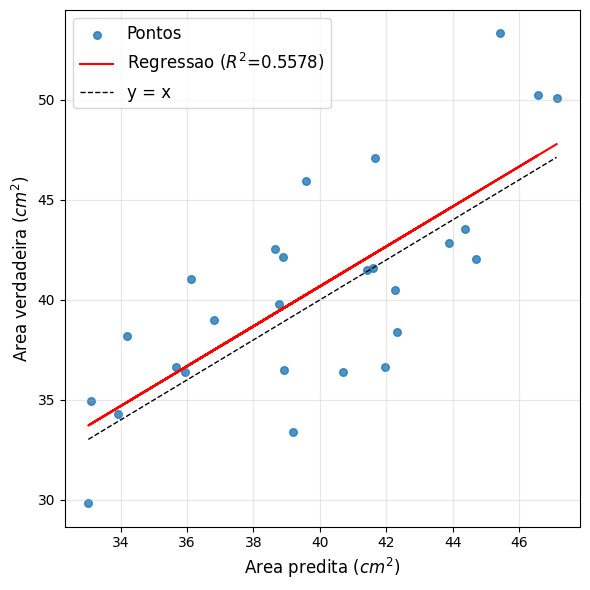
\includegraphics[width=\textwidth]{figures/cap3/rquadradounet.jpeg}
        \caption{$R^2$ entre as medidas preditas e as medidas reais da AOL.}
    \end{subfigure}
    \hfill
    \begin{subfigure}{1\textwidth}
        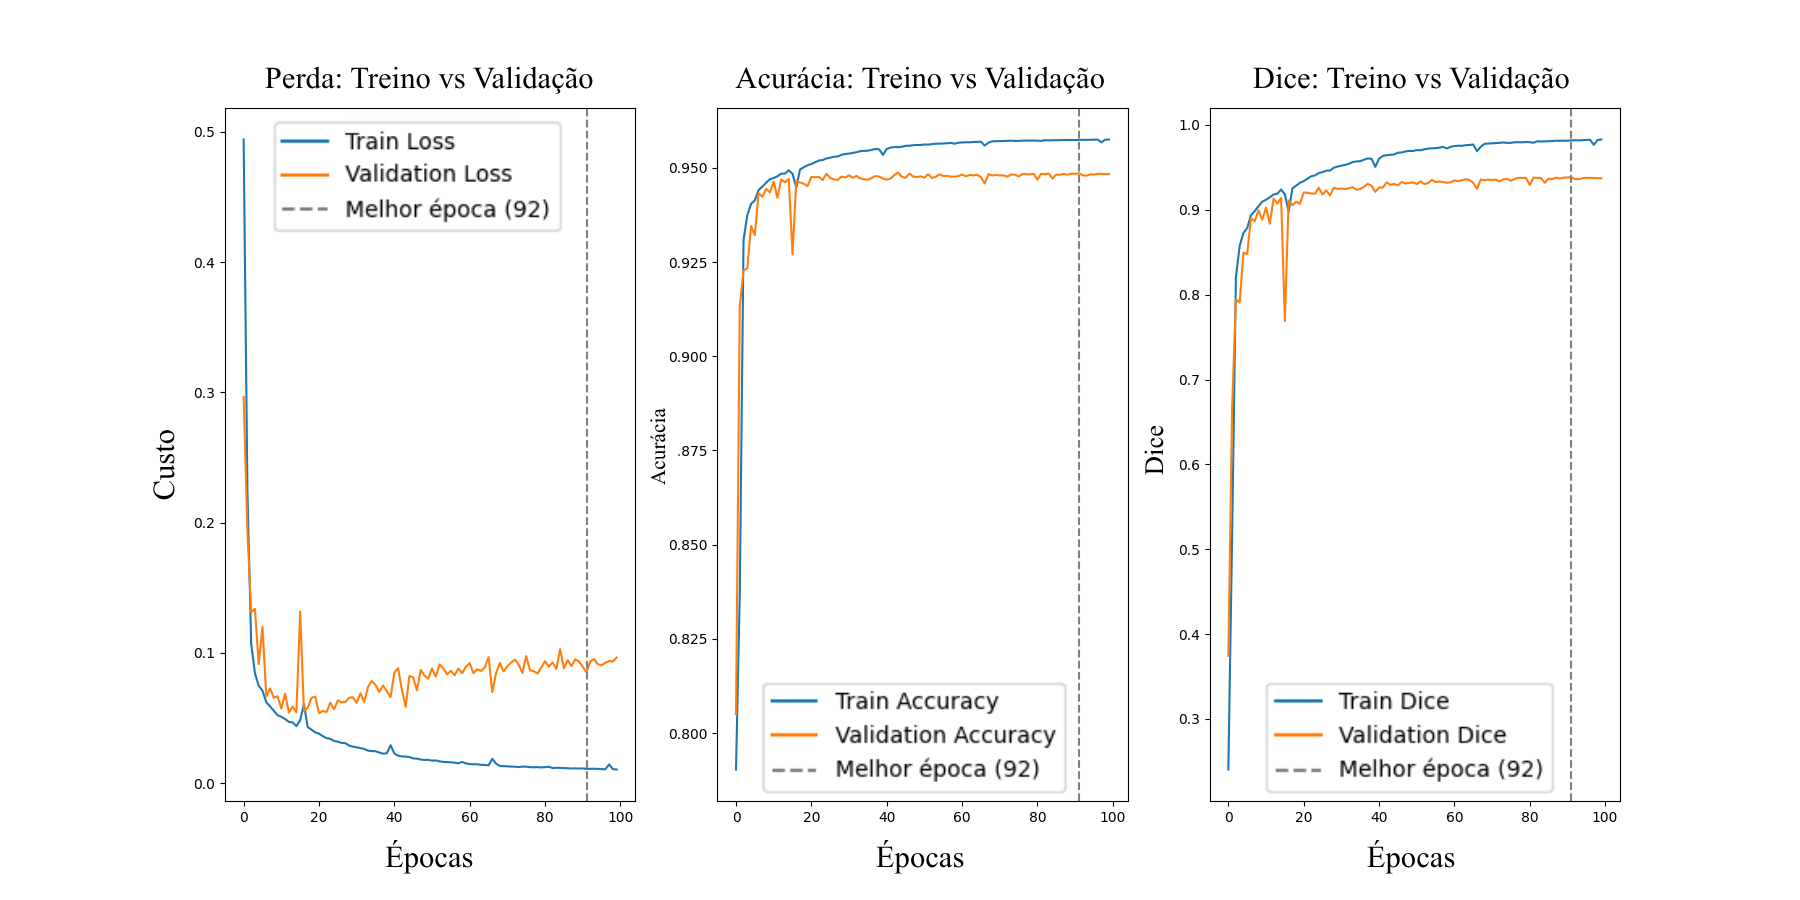
\includegraphics[width=\textwidth]{figures/cap3/AOL_Unet128_k_4.png}
        \caption{Gráficos de custo, \textit{Dice} e acurácia ao longo das épocas para o modelo de U-Net multitarefa.}
    \end{subfigure}
    \caption*{Fonte: Elaboração do Autor.}
    \label{cap3:metricasAOL}
\end{figure}


\subsubsection{U-Net Fuzzy}

Para a AOL, o modelo U-Net Fuzzy apresentou desempenho superior ao da U-Net multitarefa na maior parte das métricas analisadas. No conjunto de validação, o modelo alcançou coeficiente de Dice médio de $93,29\%$ e acurácia média de $95,15\%$, indicando melhor sobreposição entre as máscaras preditas e as máscaras de referência. A convergência ocorreu, em média, após $89$ épocas, valor superior ao observado para o modelo sem inferência fuzzy.

No que se refere às medidas numéricas, o modelo apresentou MAE de $2,312$ cm$^2$ e $R^2$ de $0,7423$, sugerindo melhor associação entre as medidas preditas e as medidas reais da AOL. No conjunto de teste, o erro máximo foi de $6,644$ cm$^2$, o erro mínimo foi de $0,225$ cm$^2$, a média predita foi de $39,865$ cm$^2$ e a média real foi de $40,559$ cm$^2$.

A Figura \ref{cap3:metricasAOL_fuzzy}(a) mostra que as medidas preditas pelo modelo fuzzy apresentaram menor dispersão em relação à reta identidade, o que é coerente com o aumento do valor de $R^2$. Na Figura \ref{cap3:metricasAOL_fuzzy}(b), observa-se que as curvas de custo, acurácia e Dice apresentaram maior oscilação ao longo do treinamento. Esse comportamento pode estar associado ao aumento de complexidade introduzido pela camada de inferência fuzzy, especialmente nas etapas iniciais do processo de otimização.

\begin{figure}[H]
    \centering
    \caption{$R^2$ entre as medidas preditas e as medidas reais da AOL e gráficos de custo, \textit{Dice} e acurácia ao longo das épocas para o modelo de U-Net Fuzzy da AOL.}
    \begin{subfigure}{0.45\textwidth}
        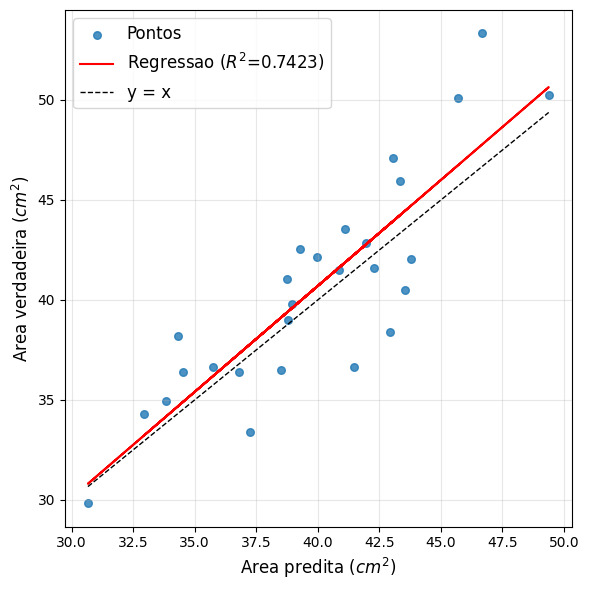
\includegraphics[width=\textwidth]{figures/cap3/rquadradofuzzy.jpeg}
        \caption{$R^2$ entre as medidas preditas e as medidas reais da AOL.}
    \end{subfigure}
    \hfill
    \begin{subfigure}{1\textwidth}
        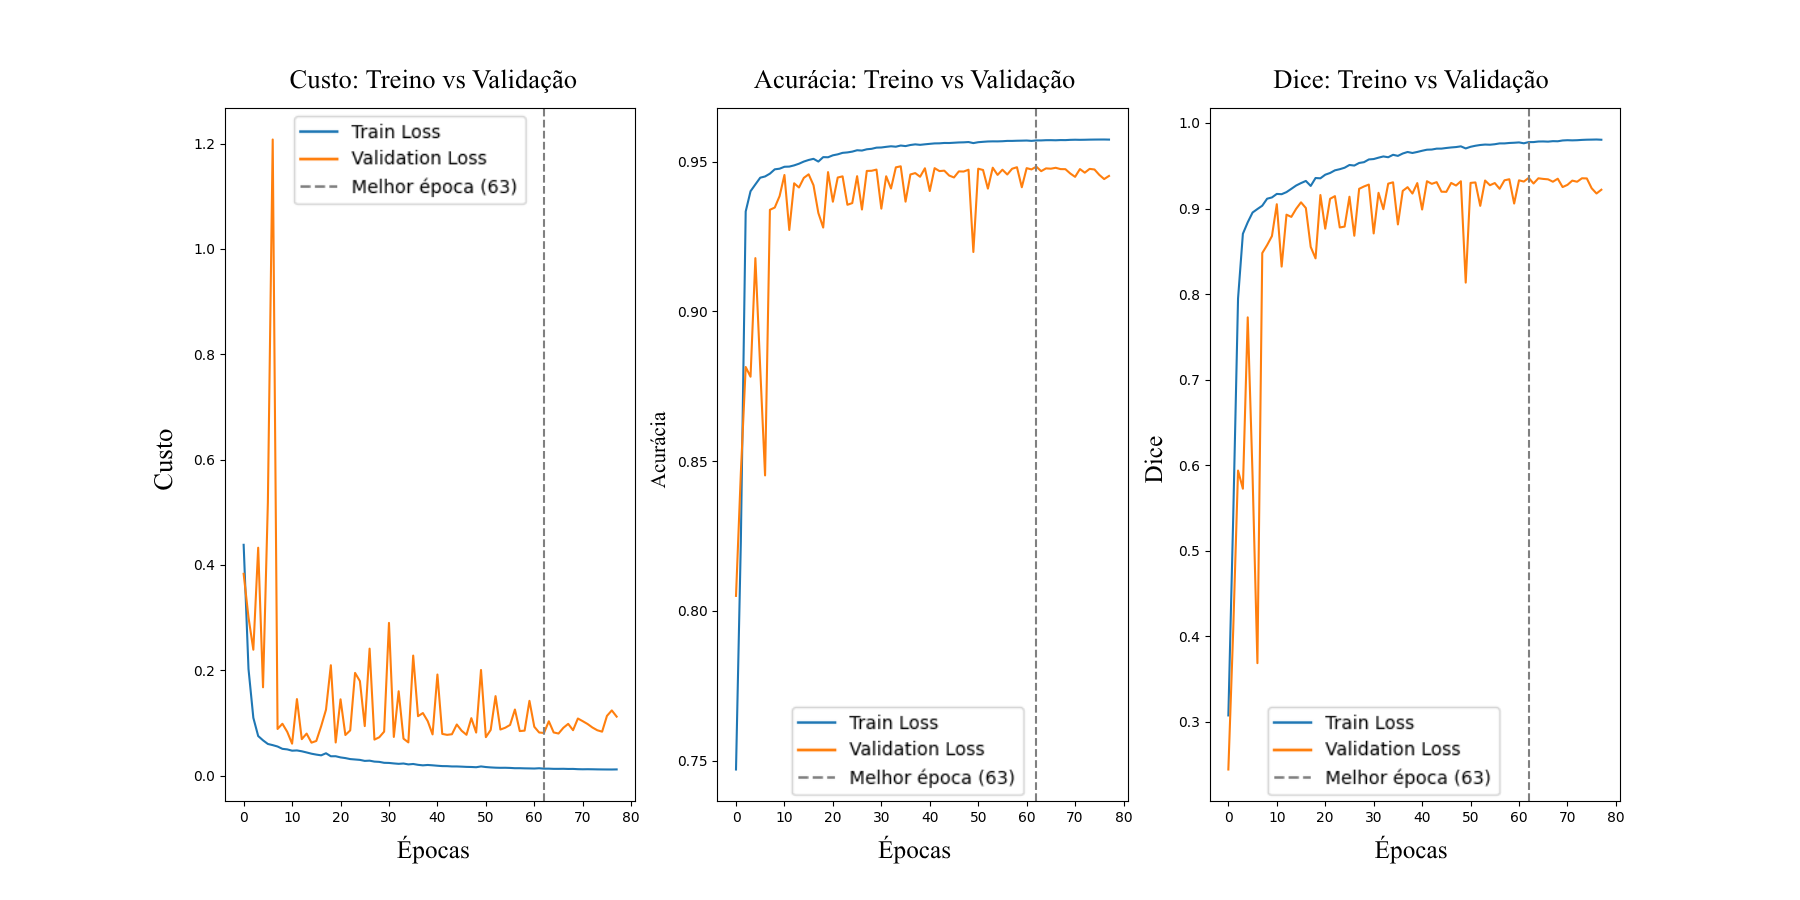
\includegraphics[width=\textwidth]{figures/cap3/AOL_fuzzy128_k_4.png}
        \caption{Gráficos de custo, \textit{Dice} e acurácia ao longo das épocas para o modelo de U-Net Fuzzy da AOL.}
    \end{subfigure}
    \caption*{Fonte: Elaboração do Autor.}
    \label{cap3:metricasAOL_fuzzy}
\end{figure}




\subsubsection{Comparação entre os modelos}

Na Tabela \ref{cap3:tabelaAOL} são resumidos os resultados obtidos para a AOL. De modo geral, o modelo U-Net Fuzzy superou o modelo U-Net multitarefa em todas as métricas principais, apresentando maior coeficiente de Dice, maior acurácia, menor erro absoluto médio e maior coeficiente de determinação. Esses resultados indicam que a integração do ANFIS contribuiu positivamente para a segmentação da região de interesse e para a extração das medidas numéricas da AOL.

Por outro lado, o modelo fuzzy demandou maior número de épocas até a convergência e apresentou maior instabilidade nas curvas de treinamento. Assim, embora tenha alcançado melhor desempenho final, seu comportamento ao longo do treinamento foi menos estável que o observado no modelo multitarefa. Ainda assim, para a tarefa de mensuração da AOL, os resultados obtidos indicam vantagem do modelo U-Net Fuzzy.

\begin{table}[H]
    \centering
    \caption{Resumo dos resultados obtidos para a AOL, comparando o modelo de U-Net multitarefa com o modelo de U-Net Fuzzy.}
    \begin{tabular}{|c|c|c|}
        \hline
        \textbf{Métrica} & \textbf{U-Net Multitarefa} & \textbf{U-Net Fuzzy} \\
        \hline
        Coeficiente de Dice & $92,73\%$ & $93,29\%$ \\
        \hline
        Acurácia & $94,75\%$ & $95,15\%$ \\
        \hline
        Número de Épocas & 80 & 89 \\
        \hline
        $R^2$ & $0,5578$ & $0,7423$ \\
        \hline
        Erro Absoluto Médio (MAE) & $2,988$ cm$^2$ & $2,312$ cm$^2$ \\
        \hline
        Erro Máximo & $7,905$ cm$^2$ & $6,644$ cm$^2$ \\
        \hline
        Erro Mínimo & $0,005$ cm$^2$ & $0,225$ cm$^2$ \\
        \hline
        Média Predita & $39,880$ cm$^2$ & $39,865$ cm$^2$ \\
        \hline
        Média Real & $40,559$ cm$^2$ & $40,559$ cm$^2$ \\
        \hline
    \end{tabular}
    \caption*{Fonte: Elaboração do Autor.}
    \label{cap3:tabelaAOL}
\end{table}



\subsection{EGL}
\subsubsection{U-Net multitarefa}
Para a mensuração da EGL, o modelo U-Net multitarefa apresentou desempenho regular na tarefa de segmentação, influênciado pela pequena quantidade de imagens disponíveis para o treinamento e pela complexidade da tarefa. No conjunto de validação, obteve coeficiente de Dice médio de $60,78\%$ e acurácia média de $99,99\%$. Observa-se que, embora a acurácia seja extremamente alta, o coeficiente de Dice é relativamente baixo, o que pode ser atribuído à dificuldade em delimitar a camada de gordura presente na região do olho de lombo, que é uma estrutura anatômica de menor dimensão e com menor contraste. Em média, a convergência do treinamento ocorreu após $88$ épocas. 


Nas médias numéricas o modelo alcançou erro absoluto médio (MAE) de $0,018$ mm e coeficiente de determinação $R^2$ igual a $0,4321$. 



Esse resultado indica que o modelo teve dificuldade em segmentar adequadamente a camada de gordura, o que comprometeu a precisão das medidas preditas. No conjunto de teste, o erro máximo observado foi de $3,456$ mm, o erro mínimo foi de $0,123$ mm, a média predita foi de $5,678$ mm e a média real foi de $6,123$ mm.

Em relação às medidas numéricas, o modelo alcançou erro absoluto médio (MAE) de $2,988$ cm$^2$ e coeficiente de determinação $R^2$ igual a $0,5578$. Esse resultado indica que, embora o modelo tenha segmentado adequadamente a região de interesse, a correspondência entre as medidas preditas e as medidas reais foi moderada. No conjunto de teste, o erro máximo observado foi de $7,905$ cm$^2$, o erro mínimo foi de $0,005$ cm$^2$, a média predita foi de $39,880$ cm$^2$ e a média real foi de $40,559$ cm$^2$

